\documentclass[ngerman]{scrartcl}
\usepackage[latin1]{inputenc}% erm\"oglich die direkte Eingabe der Umlaute 
\usepackage[T1]{fontenc} % das Trennen der Umlaute
\usepackage{ngerman}
\usepackage[decimalsymbol=comma,
            loctolang={DE:ngerman,UK:english},
            separate-uncertainty = true,
            multi-part-units=single
            ]{siunitx}
\usepackage{paralist}
\usepackage{amsmath}
\usepackage{graphicx}
\usepackage{booktabs}
\usepackage{float}
\usepackage{caption}
\usepackage{subcaption}
\usepackage{tabularx}
\usepackage{array}
\usepackage{commath}
\usepackage{amsfonts}


\title{Praktikum Klassische Physik Teil 2 (P2)}
\subtitle{Operationsverst�rker}
\author{Simon Fromme, Philipp Laur}

\date{\today}

\begin{document}

%\parindent 0pt

\maketitle
\tableofcontents
\newpage

\section{Transistorverst�rker}
\label{sec:transistorverstarker}

\subsection{gleichstromgegengekoppelte Schaltung}
\label{sec:vollst-emitt}

Die vollst�ndige Emitter-Verst�rkerschaltung wird wie in der Vorbereitungshilfe beschrieben aufgebaut, allerdings wird statt einem $\SI{5}{\micro\farad}$-Kondensator ein $\SI{4,7}{\micro\farad}$-Kondensator verwendet. Am Signalgenerator wurde eine Dreieckspannung mit der Frequenz $f=\SI{1000}{\hertz}$ erzeugt. Die gemessenen Spannungswerte am Ein- und Ausgang sind in Tabelle \ref{table:transistor1} angebeben.

\begin{table}[htbp]
\centering
\caption{Messergebnisse gleichstromgegengekoppelte Emitterschaltung}
\begin{tabular}{rr|r}
\toprule
$U_E^{SS}$ in $\si{\mV}$ & $U_A^{SS}$ in $\si{\V}$ & $\beta = \dfrac{U_A^{SS}}{U_E^{SS}}$\\ 
\midrule
26 & 4,0 & 153,85 \\ 
32 & 5,2 & 162,50 \\
42 & 7,4 & 176,19 \\  
58 & 9,8 & 168,97 \\ 
\bottomrule
\end{tabular}
\label{table:transistor1}
\end{table}

Mittelt man �ber diese Werte, so erh�lt man einen Verst�rkungsfaktor von 
\begin{align*}
  \beta = 165,38.
\end{align*}

Zu bemerken ist, dass der Verst�rkungsfaktor in einem relativ breiten Intervall schwankt, was auf eine vergleichsweise schlechte Qualit�t dieser Transistor-Verst�rkerschaltung hindeutet. Bei h�heren Eingangsspannungen scheint der Verst�rkungsfaktor etwas h�her zu liegen, jedoch l�sst die geringe Zahl der Messwerte keine genaue Aussage zu. 

\subsection{stromgegengekoppelte Schaltung}
\label{sec:stromg-schalt}

Bei der vorherigen Schaltung wird nun der Kondensator $C_E$ entfernt, was die Gegenkopplung auf den gesamten Frequenzbereich ausweitet. Die Messwerte (Tabelle \ref{table:transistor2}) werden ganz analog zur vorherigen Teilaufgabe genommen ($f = \SI{1000}{\hertz}$) und wiederum der Verst�rkungsfaktor $\beta$ bestimmt. 

\begin{table}[htbp]
\centering
\caption{Messergebnisse stromgekoppelte Emitterschaltung}
\begin{tabular}{rr|r}
\toprule
$U_E^{SS}$ in $\si{\mV}$ & $U_A^{SS}$ in $\si{\mV}$ & $\beta = \dfrac{U_A^{SS}}{U_E^{SS}}$\\ 
\midrule
25,6 & 114 & 4,45 \\ 
56,8 & 250 & 4,40 \\ 
106 & 464 & 4,38 \\ 
\bottomrule
\end{tabular}
\label{table:transistor2}
\end{table}

Zu beobachten ist hier, dass der Verst�rkungsfaktor $\beta$ einer geringeren Schwankung als bei der gleichstromgegengekoppelten Emitterschaltung unterliegt. 

Durch Mittelung �ber die Verst�rkungsfaktoren der einzelnen Messungen ergibt sich 
\begin{align*}
  \beta = 4,41.
\end{align*}
Der Verst�rkungsfaktor ist bei gleicher Frequenz von $f=\SI{1000}{\hertz}$ also wesentlich geringer als bei der gleichstromgegengekoppelten Emitterschaltung. Der Grund daf�r ist, dass der Widerstand $R_E$ f�r hohe Frequenzen nun nicht mehr durch den Kondensator $C_E$ �berbr�ckt wird, so dass an $R_E$ eine h�here Spannung abf�llt und der Emitter dementsprechend auf einem h�heren Potential liegt. Somit verringert sich die Ausgangsspannung.

\subsection{Verst�rkung in Abh�ngigkeit der Frequenz}
\label{sec:verst-abhang-der}

% Diagramme (Frequenzabh�ngige Verst�rkung)
\begin{figure}
  \centering
  \caption{Frequenzabh�ngige Verst�rkung bei Stromgegenkopplung}
  % GNUPLOT: LaTeX picture with Postscript
\begingroup
  \makeatletter
  \providecommand\color[2][]{%
    \GenericError{(gnuplot) \space\space\space\@spaces}{%
      Package color not loaded in conjunction with
      terminal option `colourtext'%
    }{See the gnuplot documentation for explanation.%
    }{Either use 'blacktext' in gnuplot or load the package
      color.sty in LaTeX.}%
    \renewcommand\color[2][]{}%
  }%
  \providecommand\includegraphics[2][]{%
    \GenericError{(gnuplot) \space\space\space\@spaces}{%
      Package graphicx or graphics not loaded%
    }{See the gnuplot documentation for explanation.%
    }{The gnuplot epslatex terminal needs graphicx.sty or graphics.sty.}%
    \renewcommand\includegraphics[2][]{}%
  }%
  \providecommand\rotatebox[2]{#2}%
  \@ifundefined{ifGPcolor}{%
    \newif\ifGPcolor
    \GPcolortrue
  }{}%
  \@ifundefined{ifGPblacktext}{%
    \newif\ifGPblacktext
    \GPblacktexttrue
  }{}%
  % define a \g@addto@macro without @ in the name:
  \let\gplgaddtomacro\g@addto@macro
  % define empty templates for all commands taking text:
  \gdef\gplbacktext{}%
  \gdef\gplfronttext{}%
  \makeatother
  \ifGPblacktext
    % no textcolor at all
    \def\colorrgb#1{}%
    \def\colorgray#1{}%
  \else
    % gray or color?
    \ifGPcolor
      \def\colorrgb#1{\color[rgb]{#1}}%
      \def\colorgray#1{\color[gray]{#1}}%
      \expandafter\def\csname LTw\endcsname{\color{white}}%
      \expandafter\def\csname LTb\endcsname{\color{black}}%
      \expandafter\def\csname LTa\endcsname{\color{black}}%
      \expandafter\def\csname LT0\endcsname{\color[rgb]{1,0,0}}%
      \expandafter\def\csname LT1\endcsname{\color[rgb]{0,1,0}}%
      \expandafter\def\csname LT2\endcsname{\color[rgb]{0,0,1}}%
      \expandafter\def\csname LT3\endcsname{\color[rgb]{1,0,1}}%
      \expandafter\def\csname LT4\endcsname{\color[rgb]{0,1,1}}%
      \expandafter\def\csname LT5\endcsname{\color[rgb]{1,1,0}}%
      \expandafter\def\csname LT6\endcsname{\color[rgb]{0,0,0}}%
      \expandafter\def\csname LT7\endcsname{\color[rgb]{1,0.3,0}}%
      \expandafter\def\csname LT8\endcsname{\color[rgb]{0.5,0.5,0.5}}%
    \else
      % gray
      \def\colorrgb#1{\color{black}}%
      \def\colorgray#1{\color[gray]{#1}}%
      \expandafter\def\csname LTw\endcsname{\color{white}}%
      \expandafter\def\csname LTb\endcsname{\color{black}}%
      \expandafter\def\csname LTa\endcsname{\color{black}}%
      \expandafter\def\csname LT0\endcsname{\color{black}}%
      \expandafter\def\csname LT1\endcsname{\color{black}}%
      \expandafter\def\csname LT2\endcsname{\color{black}}%
      \expandafter\def\csname LT3\endcsname{\color{black}}%
      \expandafter\def\csname LT4\endcsname{\color{black}}%
      \expandafter\def\csname LT5\endcsname{\color{black}}%
      \expandafter\def\csname LT6\endcsname{\color{black}}%
      \expandafter\def\csname LT7\endcsname{\color{black}}%
      \expandafter\def\csname LT8\endcsname{\color{black}}%
    \fi
  \fi
  \setlength{\unitlength}{0.0500bp}%
  \begin{picture}(7200.00,5040.00)%
    \gplgaddtomacro\gplbacktext{%
      \csname LTb\endcsname%
      \put(682,704){\makebox(0,0)[r]{\strut{} 0}}%
      \put(682,1518){\makebox(0,0)[r]{\strut{} 1}}%
      \put(682,2332){\makebox(0,0)[r]{\strut{} 2}}%
      \put(682,3147){\makebox(0,0)[r]{\strut{} 3}}%
      \put(682,3961){\makebox(0,0)[r]{\strut{} 4}}%
      \put(682,4775){\makebox(0,0)[r]{\strut{} 5}}%
      \put(956,484){\makebox(0,0){\strut{} 10}}%
      \put(2417,484){\makebox(0,0){\strut{} 100}}%
      \put(3879,484){\makebox(0,0){\strut{} 1000}}%
      \put(5341,484){\makebox(0,0){\strut{} 10000}}%
      \put(6803,484){\makebox(0,0){\strut{} 100000}}%
      \put(176,2739){\rotatebox{-270}{\makebox(0,0){\strut{}$\beta$}}}%
      \put(3808,154){\makebox(0,0){\strut{}$f$ in $\si{\Hz}$}}%
    }%
    \gplgaddtomacro\gplfronttext{%
    }%
    \gplbacktext
    \put(0,0){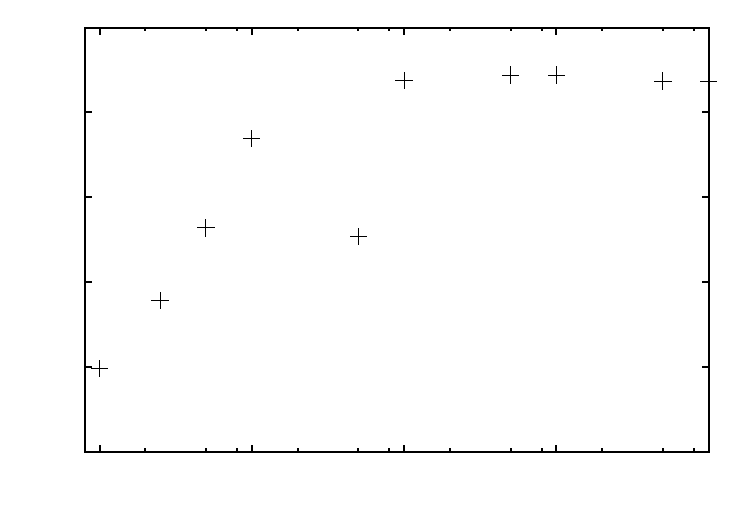
\includegraphics{Diagramme/frequenz-kopplung}}%
    \gplfronttext
  \end{picture}%
\endgroup

\end{figure}

\begin{figure}
  \centering
  \caption{Frequenzabh�ngige Verst�rkung bei Gleichstromgegenkopplung}
  % GNUPLOT: LaTeX picture with Postscript
\begingroup
  \makeatletter
  \providecommand\color[2][]{%
    \GenericError{(gnuplot) \space\space\space\@spaces}{%
      Package color not loaded in conjunction with
      terminal option `colourtext'%
    }{See the gnuplot documentation for explanation.%
    }{Either use 'blacktext' in gnuplot or load the package
      color.sty in LaTeX.}%
    \renewcommand\color[2][]{}%
  }%
  \providecommand\includegraphics[2][]{%
    \GenericError{(gnuplot) \space\space\space\@spaces}{%
      Package graphicx or graphics not loaded%
    }{See the gnuplot documentation for explanation.%
    }{The gnuplot epslatex terminal needs graphicx.sty or graphics.sty.}%
    \renewcommand\includegraphics[2][]{}%
  }%
  \providecommand\rotatebox[2]{#2}%
  \@ifundefined{ifGPcolor}{%
    \newif\ifGPcolor
    \GPcolortrue
  }{}%
  \@ifundefined{ifGPblacktext}{%
    \newif\ifGPblacktext
    \GPblacktexttrue
  }{}%
  % define a \g@addto@macro without @ in the name:
  \let\gplgaddtomacro\g@addto@macro
  % define empty templates for all commands taking text:
  \gdef\gplbacktext{}%
  \gdef\gplfronttext{}%
  \makeatother
  \ifGPblacktext
    % no textcolor at all
    \def\colorrgb#1{}%
    \def\colorgray#1{}%
  \else
    % gray or color?
    \ifGPcolor
      \def\colorrgb#1{\color[rgb]{#1}}%
      \def\colorgray#1{\color[gray]{#1}}%
      \expandafter\def\csname LTw\endcsname{\color{white}}%
      \expandafter\def\csname LTb\endcsname{\color{black}}%
      \expandafter\def\csname LTa\endcsname{\color{black}}%
      \expandafter\def\csname LT0\endcsname{\color[rgb]{1,0,0}}%
      \expandafter\def\csname LT1\endcsname{\color[rgb]{0,1,0}}%
      \expandafter\def\csname LT2\endcsname{\color[rgb]{0,0,1}}%
      \expandafter\def\csname LT3\endcsname{\color[rgb]{1,0,1}}%
      \expandafter\def\csname LT4\endcsname{\color[rgb]{0,1,1}}%
      \expandafter\def\csname LT5\endcsname{\color[rgb]{1,1,0}}%
      \expandafter\def\csname LT6\endcsname{\color[rgb]{0,0,0}}%
      \expandafter\def\csname LT7\endcsname{\color[rgb]{1,0.3,0}}%
      \expandafter\def\csname LT8\endcsname{\color[rgb]{0.5,0.5,0.5}}%
    \else
      % gray
      \def\colorrgb#1{\color{black}}%
      \def\colorgray#1{\color[gray]{#1}}%
      \expandafter\def\csname LTw\endcsname{\color{white}}%
      \expandafter\def\csname LTb\endcsname{\color{black}}%
      \expandafter\def\csname LTa\endcsname{\color{black}}%
      \expandafter\def\csname LT0\endcsname{\color{black}}%
      \expandafter\def\csname LT1\endcsname{\color{black}}%
      \expandafter\def\csname LT2\endcsname{\color{black}}%
      \expandafter\def\csname LT3\endcsname{\color{black}}%
      \expandafter\def\csname LT4\endcsname{\color{black}}%
      \expandafter\def\csname LT5\endcsname{\color{black}}%
      \expandafter\def\csname LT6\endcsname{\color{black}}%
      \expandafter\def\csname LT7\endcsname{\color{black}}%
      \expandafter\def\csname LT8\endcsname{\color{black}}%
    \fi
  \fi
  \setlength{\unitlength}{0.0500bp}%
  \begin{picture}(7200.00,5040.00)%
    \gplgaddtomacro\gplbacktext{%
      \csname LTb\endcsname%
      \put(946,704){\makebox(0,0)[r]{\strut{} 0}}%
      \put(946,1722){\makebox(0,0)[r]{\strut{} 50}}%
      \put(946,2740){\makebox(0,0)[r]{\strut{} 100}}%
      \put(946,3757){\makebox(0,0)[r]{\strut{} 150}}%
      \put(946,4775){\makebox(0,0)[r]{\strut{} 200}}%
      \put(1213,484){\makebox(0,0){\strut{} 10}}%
      \put(2611,484){\makebox(0,0){\strut{} 100}}%
      \put(4008,484){\makebox(0,0){\strut{} 1000}}%
      \put(5406,484){\makebox(0,0){\strut{} 10000}}%
      \put(6803,484){\makebox(0,0){\strut{} 100000}}%
      \put(176,2739){\rotatebox{-270}{\makebox(0,0){\strut{}$\beta$}}}%
      \put(3940,154){\makebox(0,0){\strut{}$f$ in $\si{\Hz}$}}%
    }%
    \gplgaddtomacro\gplfronttext{%
    }%
    \gplbacktext
    \put(0,0){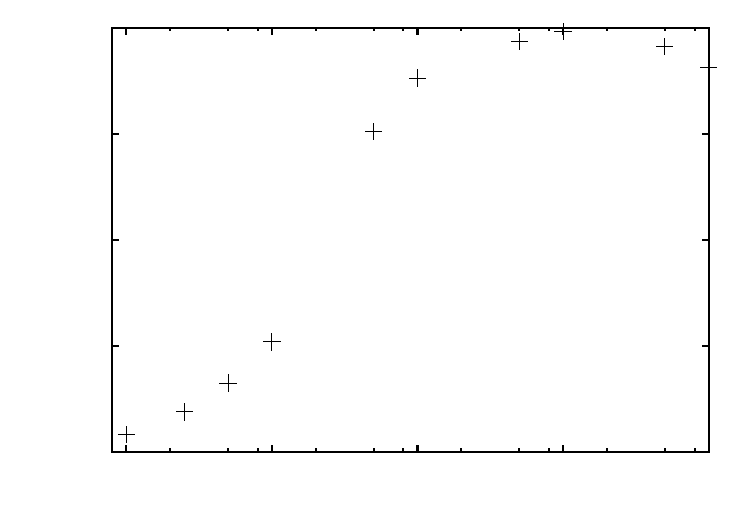
\includegraphics{Diagramme/frequenz-kopplung_gs}}%
    \gplfronttext
  \end{picture}%
\endgroup

\end{figure}




\end{document}
